% !TEX TS-program = XeLaTeX
% use the following command:
% all document files must be coded in UTF-8
\documentclass[portuguese]{textolivre}
% build HTML with: make4ht -e build.lua -c textolivre.cfg -x -u article "fn-in,svg,pic-align"

\journalname{Texto Livre}
\thevolume{19}
%\thenumber{1} % old template
\theyear{2026}
\receiveddate{\DTMdisplaydate{2025}{11}{30}{-1}} % YYYY MM DD
\accepteddate{\DTMdisplaydate{2026}{1}{26}{-1}}
\publisheddate{\DTMdisplaydate{2026}{7}{21}{-1}}
\corrauthor{Viviane Cristina Vieira}
\articledoi{10.1590/1983-3652.2026.63157}
%\articleid{NNNN} % if the article ID is not the last 5 numbers of its DOI, provide it using \articleid{} commmand 
% list of available sesscions in the journal: articles, dossier, reports, essays, reviews, interviews, editorial
\articlesessionname{dossier}
\runningauthor{Barros e Vieira} 
%\editorname{Leonardo Araújo} % old template
\sectioneditorname{Francis Arthuso Paiva~\orcid{0000-0002-9083-3342}}
\layouteditorname{Leonardo Araujo~\orcid{0000-0003-3884-2177}}

\title{Análise de vídeos de entretenimento infantil no YouTube brasileiro como ação, interação e relação no capitalismo informacional}
\othertitle{Analysis of Brazilian YouTube Children’s Entertainment Videos as Action, Interaction, and Relation in Informational Capitalism}
% if there is a third language title, add here:
%\othertitle{Artikelvorlage zur Einreichung beim Texto Livre Journal}

\author[1]{Helena Sarmento Barros~\orcid{0009-0005-6794-4713}\thanks{Email: \href{mailto:helenasarmbar@gmail.com}{helenasarmbar@gmail.com}}}
\author[1]{Viviane Cristina Vieira~\orcid{0000-0003-4148-5414}\thanks{Email: \href{mailto:vivi@unb.br}{vivi@unb.br}}}
\affil[1]{Universidade de Brasília, Instituto de Letras, Programa de Pós-Graduação em Linguística, Brasília, DF, Brasil.}

\addbibresource{article.bib}
% use biber instead of bibtex
% $ biber article

% used to create dummy text for the template file
\definecolor{dark-gray}{gray}{0.35} % color used to display dummy texts
\usepackage{lipsum}
\SetLipsumParListSurrounders{\colorlet{oldcolor}{.}\color{dark-gray}}{\color{oldcolor}}

% used here only to provide the XeLaTeX and BibTeX logos
\usepackage{hologo}

% if you use multirows in a table, include the multirow package
\usepackage{multirow}

% provides sidewaysfigure environment
\usepackage{rotating}

% CUSTOM EPIGRAPH - BEGIN 
%%% https://tex.stackexchange.com/questions/193178/specific-epigraph-style
\usepackage{epigraph}
\renewcommand\textflush{flushright}
\makeatletter
\newlength\epitextskip
\pretocmd{\@epitext}{\em}{}{}
\apptocmd{\@epitext}{\em}{}{}
\patchcmd{\epigraph}{\@epitext{#1}\\}{\@epitext{#1}\\[\epitextskip]}{}{}
\makeatother
\setlength\epigraphrule{0pt}
\setlength\epitextskip{0.5ex}
\setlength\epigraphwidth{.7\textwidth}
% CUSTOM EPIGRAPH - END

% to use IPA symbols in unicode add
%\usepackage{fontspec}
%\newfontfamily\ipafont{CMU Serif}
%\newcommand{\ipa}[1]{{\ipafont #1}}
% and in the text you may use the \ipa{...} command passing the symbols in unicode

% LANGUAGE - BEGIN
% ARABIC
% for languages that use special fonts, you must provide the typeface that will be used
% \setotherlanguage{arabic}
% \newfontfamily\arabicfont[Script=Arabic]{Amiri}
% \newfontfamily\arabicfontsf[Script=Arabic]{Amiri}
% \newfontfamily\arabicfonttt[Script=Arabic]{Amiri}
%
% in the article, to add arabic text use: \textlang{arabic}{ ... }
%
% RUSSIAN
% for russian text we also need to define fonts with support for Cyrillic script
% \usepackage{fontspec}
% \setotherlanguage{russian}
% \newfontfamily\cyrillicfont{Times New Roman}
% \newfontfamily\cyrillicfontsf{Times New Roman}[Script=Cyrillic]
% \newfontfamily\cyrillicfonttt{Times New Roman}[Script=Cyrillic]
%
% in the text use \begin{russian} ... \end{russian}
% LANGUAGE - END

% EMOJIS - BEGIN
% to use emoticons in your manuscript
% https://stackoverflow.com/questions/190145/how-to-insert-emoticons-in-latex/57076064
% using font Symbola, which has full support
% the font may be downloaded at:
% https://dn-works.com/ufas/
% add to preamble:
% \newfontfamily\Symbola{Symbola}
% in the text use:
% {\Symbola }
% EMOJIS - END

% LABEL REFERENCE TO DESCRIPTIVE LIST - BEGIN
% reference itens in a descriptive list using their labels instead of numbers
% insert the code below in the preambule:
%\makeatletter
%\let\orgdescriptionlabel\descriptionlabel
%\renewcommand*{\descriptionlabel}[1]{%
%  \let\orglabel\label
%  \let\label\@gobble
%  \phantomsection
%  \edef\@currentlabel{#1\unskip}%
%  \let\label\orglabel
%  \orgdescriptionlabel{#1}%
%}
%\makeatother
%
% in your document, use as illustraded here:
%\begin{description}
%  \item[first\label{itm1}] this is only an example;
%  % ...  add more items
%\end{description}
% LABEL REFERENCE TO DESCRIPTIVE LIST - END


% add line numbers for submission
%\usepackage{lineno}
%\linenumbers

\begin{document}
\maketitle

\begin{polyabstract}
\begin{abstract}
Neste artigo, apresentamos resultados da pesquisa “A brincadeira do invisível: recursos discursivos multimodais no entretenimento infantil mediado pelo Youtube”, que objetiva analisar formas e modos de interação em vídeos de entretenimento infantil no YouTube brasileiro com base na Análise do Discurso Crítica \cite{Fairclough2003AnalysingDiscourse,VieiraResende2016AnaliseDiscursoCritica,Vieira2024Decolonial}. No artigo, especificamente, apresentamos um exemplo de análise do vídeo “Não fale o nome do monstro”, do Canal YouTube Enaldinho, observando os principais processos multissemiótico-discursivos como: affordance, indexação, meta-conteúdo, estruturas visuais e esquema modular, ethos discursivo, bem como intertextualidade \cite{Benson2016DiscourseYouTube,ColetivaCiborga2022EtnografiaDigital,Fairclough2003AnalysingDiscourse,KressVanLeeuwen2020ReadingImages,Maingueneau2020GenerosWeb}. A análise discursivo-crítica é parte de um estudo qualitativo documental digital \cite{Paveau2021AnaliseDiscursoDigital} que busca investigar como os sentidos são produzidos, distribuídos e naturalizados por meio da combinação de múltiplos modos semióticos – imagem, vídeo, som, layout e outros – e como essas construções podem participar da formação de subjetividades infantis e da reprodução de ideologias. Os resultados da pesquisa mais ampla indicam que, em um ambiente interacional mediado e marcado por algoritmos e estratégias de engajamento orientadas por métricas de engajamento, característico do capitalismo informacional \cite{Han2018Psicopolitica}, os recursos discursivos mobilizados no YouTube infantil incorporam lógicas e formas de expressão típicas do universo digital adulto, suplantando o imaginário próprio da infância por modelos de consumo e engajamento moldados pelas mesmas práticas mercadológicas direcionadas a pessoas adultas. Conclui-se que, ao condicionar o conteúdo produzido na plataforma, a \textit{affordance} do Youtube age como coautora dos discursos nela veiculados.

\keywords{Análise de discurso crítica \sep Semiótica social \sep YouTube \sep Multimodalidade \sep Algoritmo}
\end{abstract}

\begin{english}
\begin{abstract}
This article presents results from the research The Invisible game: multimodal-discursive resources in children’s entertainment mediated by Youtube, which aims to analyze forms and modes of interaction and social relation in Brazilian children’s entertainment videos on YouTube, based on Critical Discourse Analysis \cite{Fairclough2003AnalysingDiscourse,VieiraResende2016AnaliseDiscursoCritica,Vieira2024Decolonial}. Specifically, the article analyzes the video “Não fale o nome do monstro”, from the YouTube channel Enaldinho, examining key multisemiotic–discursive processes such as affordance, indexicality, meta-content, visual structures and modular schemes, discursive ethos, and intertextuality \cite{Benson2016DiscourseYouTube,ColetivaCiborga2022EtnografiaDigital,Fairclough2003AnalysingDiscourse,KressVanLeeuwen2020ReadingImages,Maingueneau2020GenerosWeb}. The study follows a qualitative digital-documentary method \cite{Paveau2021AnaliseDiscursoDigital} to investigate how meanings are produced, distributed, and naturalized through the combination of multiple semiotic modes – image, video, sound, layout, and others – and how such constructions may shape children’s subjectivities and reproduce ideologies. The results indicate that, within an interactional environment mediated and shaped by algorithms and engagement-driven metrics characteristic of informational capitalism \cite{Han2018Psicopolitica}, the discursive resources mobilized in children’s YouTube content incorporate logics and expressive forms typical of the adult digital universe, supplanting childhood imaginaries with consumption- and engagement-oriented models derived from adult practices. The study concludes that, by deeply conditioning the content produced on the platform, YouTube’s affordance operates as a co-author of the discourses it circulates.

\keywords{Critical discourse analysis \sep Social semiotics \sep YouTube \sep Multimodality \sep Algorithm}
\end{abstract}
\end{english}
% if there is another abstract, insert it here using the same scheme
\end{polyabstract}

\section{Introdução}\label{sec-intro}
Vídeos voltados para o entretenimento de crianças compõem uma parte substancial do catálogo do YouTube. A plataforma tornou-se um dos principais meios de recreação infantil na contemporaneidade. A pesquisa TIC Kids Online Brasil \cite{CGI2025TICKidsOnline2024} reportou que, entre crianças brasileiras de 6 a 12 anos, 70,4\% usam dispositivos eletrônicos para acessar o YouTube diariamente, enquanto 17,1\% o fazem várias vezes por semana, demonstrando alta prevalência do seu uso para lazer.
 	
Esse consumo de entretenimento é característico do contexto da psicopolítica \cite{Han2018Psicopolitica}, em que dispositivos digitais operam como vetores de colonização da subjetividade, reorganizando práticas sociais a partir da exploração emocional e afetiva dos sujeitos. Está, ainda, localizado no que \textcite{Castells2000RiseNetworkSociety} e outros definem como sociedade da informação, em que fluxos comunicacionais são mediados por plataformas algorítmicas com grande capacidade de moldar percepções, discursos e modos de inter-ação. \textcite{Castells2000RiseNetworkSociety} argumenta que a tecnologia da informação trouxe uma nova lógica em rede de organização social, culminando em uma tendência histórica na qual as principais funções e processos das nações avançadas são cada vez mais organizados em torno de redes. Essa lógica “induz uma determinação social de nível mais elevado do que a dos interesses sociais específicos expressos por meio das redes: o poder dos fluxos prevalece sobre os fluxos de poder” \cite[p. 500]{Castells2000RiseNetworkSociety}.

Em sua ubiquidade, o conteúdo veiculado no Youtube ocupa um lugar de relevância na construção de repertórios culturais e imaginários infantis, com potencial para influenciar padrões de consumo, formas de sociabilidade e identificações subjetivas. Por sua vez, o discurso tem alto potencial para a naturalização do agir mercadológico da interação digital organizada por algoritmos e direcionada a crianças, que estão numa posição de suscetibilidade à influência midiática. Para além da publicidade, o YouTube também extrai valor de parcerias institucionais e da própria estrutura de monetização por assinatura (o YouTube Premium), em que o modelo se desloca da publicidade para a lógica de retenção de usuários. Em todos os casos, o funcionamento da plataforma depende de um sistema opaco de seleção algorítmica. \textcite{Gillespie2018CustodiansInternet} discute como essa curadoria automatizada (e, por isso, de aparente neutralidade) molda o discurso público e favorece determinados formatos enquanto inibe outros, se transformando no elemento central da mediação de conteúdo por plataformas digitais. Limites técnicos, como a duração dos vídeos postados, bem como as regras que definem quem pode ultrapassar esses limites e quem não pode, “estabelecem uma hierarquia escalonada entre os produtores de conteúdo” \cite[p. 189, tradução própria]{Gillespie2018CustodiansInternet}.

Assim, produtos audiovisuais voltados à infância veiculados no Youtube compõem este ecossistema de produção, circulação e monetização altamente dependente de parâmetros computacionais e decisões corporativas globais: o conteúdo nasce da negociação entre a criatividade e os imperativos algorítmicos.

“Algoritmo” é um termo amplo: pode referir-se de modo geral a “procedimentos codificados para transformar dados de entrada em uma saída desejada, com base em cálculos especificados” \cite[p. 1]{Gillespie2018CustodiansInternet}. Neste estudo, refere-se especificamente aos sistemas de recomendação baseados em aprendizagem de máquina, como os do YouTube. São ferramentas de inteligência artificial, porque apreendem padrões de comportamento e adaptam as previsões. Trata-se de uma ferramenta preditiva automatizada que se ajusta aos sinais de engajamento (tempo de visualização, número de cliques, retenção), e assim estabelece quais formatos narrativos, elementos visuais, sonoros e gestuais ganham preferência de visualização na plataforma. Os algoritmos participam, portanto, da interação online ao selecionar e impor quem vê o quê, moldando assim quais recursos multimodais ganham tração e quais permanecem marginalizados. \textcite{AraujoAraujo2024RacismoAlgoritmico} destacam a importância da Inteligência Artificial (IA) e dos algoritmos preditivos no discurso digital:

\begin{quote}
    A IA desempenha um papel crescente na sociedade, influenciando decisões em áreas como saúde, crédito e justiça criminal. No entanto, a suposta neutralidade dos algoritmos se revela questionável ao analisarmos os padrões e preconceitos nos dados usados para treiná-los, contribuindo para a desinformação (Prado, 2022) e ameaçando a desigualdade e a democracia (O’Neil, 2020). A questão do racismo algorítmico é especialmente preocupante, pois a IA frequentemente reproduz e amplifica estereótipos e preconceitos existentes na sociedade \cite[p. 90]{AraujoAraujo2024RacismoAlgoritmico}.
\end{quote}

A respeito da influência algorítmica sobre o conteúdo veiculado no Youtube, \textcite{Adami2009VideoInteraction} passou a monitorar o módulo "Vídeos Mais Respondidos" (\textit{charts}), ao longo de um período de catorze meses, para identificar tendências de visibilidade. Utilizando gráficos de distribuição, Adami demonstra uma mudança de influência algorítmica: a transição de conteúdos com temas específicos para conteúdos mais generalistas, gerada pela própria disposição interacional da plataforma:

\begin{quote}
    Como […] a incidência de solicitações de vídeos (específicos por tópico) diminuiu ao longo do período de monitoramento, em favor de vídeos mais genéricos […], essa aparente ‘incoerência’ pode ser considerada uma característica distintiva de como a relação de redirecionamento é construída nas trocas interacionais mediadas por vídeo \cite[p. 105, tradução própria]{Adami2009VideoInteraction}.
\end{quote}

Os dados gerados por Adami já são, no momento presente, documento histórico: a interface do Youtube se transformou incrementalmente ao longo dos anos, e atualmente o módulo que costumava se dedicar a exibir os vídeos mais respondidos não está mais na interface da plataforma. Contudo, longe de obsoleto, o fenômeno descrito por Adami continua, hoje, evidente na interface da plataforma.

A precoce observação de Adami sobre a falta de controle do usuário sobre os algoritmos da plataforma ressoa na investigação de \textcite{YuEtAl2024YouTubeRecommendations}, que em experimento com usuários reais e em escala considerável demonstraram como intervenções computacionais podem ajustar os algoritmos do YouTube para combater a tendência de sugerir apenas conteúdos de entretenimento, de desinformação ou ideologicamente extremos. Ao reproduzir vídeos de notícias ideologicamente equilibradas em segundo plano, os pesquisadores conseguiram "dar um empurrão" (\textit{nudging}) no algoritmo, resultando em um aumento sustentável na oferta de informações diversas e na redução de bolhas partidárias, especialmente entre os usuários conservadores. O \textit{nudging} foi realizado pelo próprio usuário ao selecionar ativamente conteúdos noticiosos no Youtube. Os resultados demonstram que alterar a entrada de dados do algoritmo é muito mais eficaz para diversificar a dieta informacional do que ações do usuário sobre a plataforma. Conforme os autores,

\begin{quote}
    Embora o comportamento dos usuários dentro da plataforma e as recomendações de conteúdo estejam intrinsecamente relacionados, os algoritmos parecem importar mais para o consumo de informação dos usuários do que aquilo que os usuários consomem importa para os algoritmos \cite[p. 8, tradução própria]{YuEtAl2024YouTubeRecommendations}.
\end{quote}

A atividade reguladora do algoritmo parte, evidentemente, da coleta de dados dos usuários. Esta questão é especialmente sensível no que diz respeito ao conteúdo infantil, porque significa que o sistema de recomendação se baseia no monitoramento da atividade online de crianças. \textcite{Barbosa2020CreatorsOperators} apresenta múltiplas implicações dessa problemática analisando as transformações no ecossistema de conteúdo infantil do YouTube após a aplicação rigorosa da regra COPPA (\textit{Children's Online Privacy Protection Act}). Como solução, o YouTube implementou um sistema que obrigou os donos de canais a identificar se seu conteúdo era "feito para crianças". A autora identifica que a nova interpretação da lei transferiu o ônus da conformidade legal para os criadores, tratando-os como "operadores" sujeitos a multas civis pesadas (até US\$ 42.530 por violação). Os efeitos da medida significaram, para criadores de conteúdo infantil, perda significativa da receita de anúncios personalizados, reduzindo drasticamente a monetização de seus canais. Como consequência,

\begin{quote}
    Criadores no YouTube podem se abster de iniciar ou continuar a produzir conteúdo infantil, seja abandonando seus canais, seja mudando suas estratégias de conteúdo para um público mais velho. Esses efeitos foram particularmente críticos para mulheres e criadores menores, o que pode intensificar o problema da desigualdade de gênero na plataforma e beneficiar grandes empresas \cite[p. 117]{Barbosa2020CreatorsOperators}.
\end{quote}

As evidências de \textcite{Adami2009VideoInteraction,YuEtAl2024YouTubeRecommendations}, bem como a problemática de regulação trazida por \textcite{Barbosa2020CreatorsOperators} acerca do papel ativo dos sistemas algorítmicos da plataforma no condicionamento da visibilidade, se materializam discursivamente nos vídeos cujo conteúdo melhor atende ao regime de visibilidade do Youtube. Essa operação é realizada por meio dos recursos semióticos concretos que estruturam a interface e também nos vídeos de \textit{megayoutubers}, que estrategicamente constroem seu conteúdo de modo a alcançar popularidade máxima. Assim, o regime técnico-operacional em questão é responsável por delimitar as formas que seus usuários humanos, tanto criadores de conteúdo quanto usuários \textit{viewers}, podem utilizar a linguagem.

Assim como é próprio do regime discursivo do mundo \textit{online}, a linguagem no Youtube é multimodal: a plataforma permite a combinação de diferentes recursos semióticos, como vídeo, imagem e texto escrito organizados em módulos \cite{Benson2016DiscourseYouTube}: descrições, \textit{cards} interativos, comentários e \textit{thumbnails} (fotos de perfil). Essa multiplicidade e densidade modal \cite{Norris2009ModalDensity} não apenas ampliam a experiência do expectador, mas também influenciam a forma como o discurso é construído, disseminado e recebido. Trata-se de uma estrutura em que a linguagem figura como sistema semiótico específico, com opções lexicais, gramaticais, semânticas e outras \cite[p. 14]{VieiraResende2016AnaliseDiscursoCritica}, que se manifesta no Youtube como textos múltiplos e simultâneos na forma visual (estática e em movimento), verbal oral, verbal escrita, gestual e sonora. Assim, não só o vídeo em si se configura como evento interacional (texto), mas também a própria página digital do Youtube se apresenta como parte do texto, como um subgênero discursivo situado.

No centro dessa estrutura está o \textit{hiperlink}, que é, simultaneamente, um gesto operacional e uma ferramenta de semiose. É o motor da máquina atencional da plataforma: conecta vídeos, ativa \textit{playlists}, promove produtos, canaliza inscritos, aciona interações cruzadas entre redes e, sobretudo, mantém o usuário retido na plataforma. Como parte irredutível da \textit{affordance}, o \textit{hiperlink} compõe o regime de visibilidade da plataforma, profundamente entrelaçado com sua estrutura comercial, e cujo efeito é moldar o conteúdo nela veiculado. Os comandos vocais característicos de \textit{youtubers} (exemplos: “se inscreve no canal!” / “ativa o sininho!” / “dá seu like!”) são uma das diversas manifestações da influência do \textit{hiperlink} sobre o conteúdo na plataforma.

Posto o potencial de influência do algoritmo sobre o conteúdo mediado por plataformas, estudamos as formas sistemáticas como essa ação se apresenta na prática, ou seja, como o algoritmo atua em certos contextos e como reverbera no discurso de cada vídeo em seu contexto situado. Por isso, analisamos \textit{como se organiza a interação discursiva no YouTube infantil e de que maneira a identificação da infância é potencialmente construída nesse nicho}. Essas questões visam compreender como a plataforma pode agir para moldar experiências infantis; como diferentes discursos se articulam para interagir com esse público e, em última instância, como a plataforma digital pode construir uma representação de infância e do que é “ser criança” na dinâmica discursiva digital.

Com base em \textcite[p. 105]{Vieira2024Decolonial}, procedemos à \textit{análise discursiva relacional-dialética da prática social particular em estudo}, em relação dialética com \textit{as redes conjunturais de práticas sociais; à análise estrutural da ordem do discurso}, pela identificação das articulações dialéticas entre redes de gêneros discursivos, discursos e estilos-vozes em práticas sociais, e à \textit{análise interacional-textual empírica de textos-interações sociais}. Neste caso, de um exemplo de vídeo do Youtube destinado ao público infantil.

A análise dos aspectos interacionais e relacionais dos eventos sociais como material empírico (e seus gêneros discursivos situados, discursos e interdiscursos materializados, assim como a ética intersubjetiva em exercício) permite o estudo material situado das conexões entre mecanismos discursivos e práticas sociais. Conforme \textcite{ChouliarakiFairclough1999DiscourseLateModernity}, a análise interacional articula duas partes: a \textit{compreensão} (ou seja, as descrições e interpretações) e a \textit{explanação}, a qual opera na interface entre conceitos e material empírico. Na explanação, analisamos textos-interações particulares com base em um arcabouço teórico particular com a finalidade de “mostrar como o momento discursivo trabalha na prática social, do ponto de vista de seus efeitos em lutas hegemônicas e relações de dominação” \cite[p. 67]{ChouliarakiFairclough1999DiscourseLateModernity}.

Para a análise do aspecto acional-relacional de gêneros discursivos situados em eventos sociais-interacionais concretos, \textcite[p. 70]{Fairclough2003AnalysingDiscourse} considera fundamental pesquisar a \textit{atividade social principal, as relações sociais e as tecnologias de comunicação} ligadas aos gêneros discursivos em estudo, de modo a considerar o que as pessoas estão fazendo; as relações sociais entre elas; assim como os modos básicos de interação e suas tecnologias, sejam elas: face a face; mediadas (carta, \textit{e-mail}, conversa telefônica); quase mediadas (livros, jornais, rádio, TV) e mediadas \textit{online} (sites, plataformas, redes sociais e suas tecnologias) \cite{Thompson2018InteracaoMediada}.

\section{Conjuntura sociotécnica interacional}\label{sec-normas}
A mediação do Youtube sobre o entretenimento infantil significa, em seu macrocontexto, uma mediação por \textit{big techs}. Definindo-as como “as grandes empresas associadas a plataformas de uso intensivo de dados” \cite[p. 148]{Morozov2018BigTech} e entendendo nesse grupo companhias como Meta, Amazon, Microsoft e Google (detentora atual do YouTube), localiza-se o fenômeno do YouTube infantil nessa infraestrutura técnica regida de forma extraterritorial, orientada por métricas automatizadas em que o lucro é gerado por meio da captura da atenção. No território das \textit{big techs}, todo o conteúdo, incluindo o direcionado à infância, é produzido, composto e distribuído por filtros algorítmicos que priorizam retenção, cliques e tempo de tela, cuja forma se molda de maneira responsiva aos indicadores de desempenho da plataforma.

A operação comercial das \textit{big techs} baseia-se na extração, no processamento e comercialização de dados em larga escala. Os espaços publicitários, note-se, são parte essencial da geração de receita das plataformas assim como são para a mídia \textit{offline}, mas o cerne de seu poder está na capacidade de captar, organizar e prever comportamentos a partir do rastreamento contínuo de atividades \textit{online}. \textcite{Zuboff2019SurveillanceCapitalism} chama isso de “capitalismo de vigilância”: o modelo em que dados comportamentais são transformados em mercadoria e comercializados como instrumentos de previsão e controle. Plataformas, como as citadas anteriormente, funcionam como sistemas de vigilância em diferentes roupagens como redes sociais, lojas ou motores de busca. O lucro vem da venda dessa vigilância às empresas anunciantes, que pagam para acessar públicos segmentados com alto grau de precisão.

Atualmente vivemos no mundo digital o modelo \textit{freemium}, em que o acesso do usuário aos recursos da plataforma é integralmente gratuito (já que “pagamos” cedendo nossos dados). \textcite{Morozov2018BigTech} considera possível que o \textit{freemium} se trate de uma fase transitória da atividade das \textit{big techs}:

\begin{quote}
    É bem possível que o modelo \textit{freemium} – exaltado por muitos como o advento de um novo tipo de capitalismo, humanitário, protetor e benéfico para os pobres – tenha se revelado, na verdade, apenas uma etapa transitória e muito incipiente da transformação digital. No fim das contas, uma economia baseada em cobranças onipresentes, calculadas de acordo com o uso efetivo e com os preços de mercado vigentes, é bem mais congruente em relação a várias outras tendências (entre as quais a ascensão do rentista) do capitalismo financeiro contemporâneo. O bem-estar digital privatizado, saudado por muitos como o início do pós- capitalismo, mais parece um afastamento radical – por isso de curto prazo – dessa tendência \cite[p. 154]{Morozov2018BigTech}.
\end{quote}

De fato, o Youtube e outras plataformas já contam com serviços de assinaturas, que eximem o usuário pagante de assistir a publicidades compulsórias antes, durante e após os vídeos. O caso do YouTube é paradigmático do modelo de negócios das \textit{big techs}: a plataforma remunera criadores de conteúdo com uma fração da receita publicitária enquanto controla todo o sistema de exibição, distribuição e monetização. No Youtube, o algoritmo recomenda vídeos, regulando a visibilidade de conteúdos e definindo, na prática, o alcance que cada vídeo postado terá. Sua arquitetura tecnológica está voltada para manter o espectador o maior tempo possível na plataforma, acumulando seus dados em contrapartida e expondo-o a anúncios personalizados. Mesmo o usuário assinante cede à plataforma seu tempo, atenção e rastros digitais. O conteúdo, nesse modelo de interação mediada \textit{online}, serve como recurso retórico de sedução publicitária.

Conforme \textcite{Thompson2018InteracaoMediada}, para além das três formas tradicionais e básicas de interação (interação face a face; interação mediada e quase interação mediada), hoje precisamos estudar os tipos de interação que se desenvolvem em ambientes digitais, mediados por tecnologias de comunicação. Para o autor, a interação mediada \textit{online}, caracterizada pelo dialogismo e abertura, permite que pessoas se conectem em amplas redes de destinatários, a exemplo das redes sociais, cujas interações são mediadas por dispositivos e podem ser acessadas por um público diversificado. Essa nova forma de interação acarretou muitas mudanças informacionais e simbólicas nos modos como as pessoas se comunicam e interagem no espaço e no tempo:

\begin{quote}
    A revolução digital, a proliferação de novas redes de comunicação e o fluxo de informações só exacerbaram esses desenvolvimentos, criando um ambiente de informação no qual o vazamento de informações e a divulgação de ações e eventos anteriormente ocultos são um risco e uma ameaça constantes. Nesse aspecto, a revolução digital não alterou meu modo de pensar sobre essas questões. Mas lembrou a todos nós quão frágil essa arena é agora, quão fluida a fronteira entre a vida pública e a vida privada se tornou atualmente e quão importante é para nós, como cientistas sociais, tentar entender esse novo turbulento mundo de visibilidade mediada na era digital \cite[p. 43]{Thompson2018InteracaoMediada}.
\end{quote}

Analisar um texto digital exige ferramentas específicas para estudo de seus elementos e formas de interação “nativas”. Assim, a escolha metodológica se ancora na análise do discurso digital, entendida aqui como o conjunto de procedimentos capazes de descrever e interpretar enunciados produzidos diretamente no ambiente \textit{online}:

\begin{quote}
    A análise do discurso digital consiste na descrição e análise do funcionamento das produções linguageiras nativas da internet, particularmente da web 2.0, em seus ambientes de produção, mobilizando igualmente os recursos linguageiros e não linguageiros dos enunciados elaborados. Chamamos de nativas as produções elaboradas on-line, nos espaços de escrita e com as ferramentas propostas pela internet, e não aquelas transpostas para o espaço digital conectado após a digitalização de espaços escriturais e editoriais pré-digitais. A análise do discurso digital cria dispositivos metodológicos e teóricos que podem dar conta do funcionamento específico dos discursos nativos da internet \cite[p. 57]{Paveau2021AnaliseDiscursoDigital}.
\end{quote}

Ao optar por uma abordagem nativa de análise do discurso \textit{online}, este trabalho se alinha a uma concepção de linguagem que não separa rigidamente o que é “da linguagem” e o que é “do ambiente”. Assume-se que, no digital, forma e conteúdo são indissociáveis, conforme \textcite[p. 58]{Paveau2021AnaliseDiscursoDigital}:

\begin{quote}
    A análise do discurso digital está baseada em uma noção simétrica que tem por objetivo discutir as concepções logocêntricas da linguística (Paveau 2009; Dias, Paveau 2016b orgs.). Uma linguística simétrica confere um lugar equivalente ao linguageiro e ao não-linguageiro na análise linguística, partindo de uma concepção compósita da língua e do discurso. Ela questiona a distinção entre o linguístico e o extralinguístico, estabelecendo um contínuo entre as matérias linguageiras e seus ambientes de produção. É esse contínuo que é colocado como objeto para a análise, e não mais apenas suas matérias linguageiras. Nesse sentido, a análise do discurso digital é uma ecologia do discurso.
\end{quote}

Entre os diversos elementos nativos de textos digitais, este trabalho se dedica aos dois que se mostraram decisivos para compreender o funcionamento discursivo do YouTube: o \textit{hiperlink} e o algoritmo. A seguir, esses dois elementos são apresentados levando em consideração suas especificidades no YouTube, de modo a situar conceitualmente o texto analisado e seus elementos constitutivos. É importante destacar que, além da publicidade, o YouTube também extrai valor de parcerias institucionais, de contratos com grandes produtoras e da própria estrutura de monetização por assinatura (o YouTube Premium), em que, para além da publicidade voltada para a retenção de usuários, ganha outras fontes de geração de lucro.

Em todos os casos, o funcionamento da plataforma depende de um sistema opaco de seleção algorítmica. \textcite{Gillespie2018CustodiansInternet} discute como essa curadoria automatizada (e, por isso, de aparente neutralidade) molda o discurso público, favorecendo determinados formatos, inibindo outros e criando um ambiente onde o poder de engajamento se sobrepõe a outros critérios. No caso específico do Youtube,

\begin{quote}
    Os formatos de vídeo e os protocolos de codificação exigidos pelo YouTube determinam o quão acessível o site é para produtores de conteúdo e para espectadores com diferentes tipos de ferramentas, e podem, sutilmente, moldar os próprios vídeos. Limites técnicos, como a duração dos vídeos postados, e as regras que definem quem pode ultrapassar esses limites e quem não pode, estabelecem uma hierarquia escalonada entre os produtores de conteúdo \cite[ p. 189, tradução própria]{Gillespie2018CustodiansInternet}.
\end{quote}

Assim sendo, produtos audiovisuais voltados à infância veiculados no Youtube compõem este sistema mercadológico monopolizado de produção, circulação e monetização altamente dependente de parâmetros computacionais e decisões corporativas globais: o conteúdo nasce da negociação entre a criatividade e os imperativos algorítmicos. Se inicialmente os vídeos do Youtube eram predominantemente amadores, caracterizados por produções simples e com baixo investimento técnico \cite{CunninghamCraig2019SocialMediaEntertainment}, hoje a plataforma consolida-se como um modelo de negócio midiático altamente estruturado.

\textcite{Kim2012InstitutionalizationYouTube} aponta que a trajetória do Youtube reflete um processo de institucionalização progressiva, em que o conteúdo gerado por usuário (\textit{user based content}, doravante UBC), embora ainda persista como marca da plataforma, coexiste com conteúdo gerado profissionalmente (\textit{professionaly based content}, doravante PBC). \textit{Youtubers} reconhecidos são, hoje, verdadeiras agências de comunicação integradas que operam com grande desenvoltura em articular produção audiovisual, \textit{marketing} digital e estratégias de monetização, capazes de empregar estratégias sofisticadas de maximização de engajamento e retenção de audiência.

Apesar disso, é possível encontrar no Youtube canais dos mais diversos tamanhos de alcance e níveis de infraestrutura de produção. Há um cenário espectral que vai desde pequenos produtores de conteúdo a agências tradicionais de mídia, oriundas da televisão, do rádio e do cinema, cujos conteúdos estão conectados pelo algoritmo: um pequeno canal doméstico e o \textit{broadcasting} de um gigante das notícias podem estar a um \textit{hiperlink} de distância.

Contudo, sabemos que o algoritmo privilegia e recompensa o conteúdo mais apto a reter a atenção, criando um ciclo de retroalimentação em que conteúdos com mais visualizações serão mais recomendados. Este entendimento reitera a perspectiva crítica desta pesquisa, assumindo que nesse campo existem “tensões hegemônicas resultantes da formação de um novo cenário mediático” \cite[p. 54]{Kim2012InstitutionalizationYouTube}.

A ascensão de \textit{megayoutubers}, criadores com dezenas de milhões de inscritos e poder de alcance equiparável ao de celebridades da mídia tradicional é um dos fenômenos da história do Youtube e têm seu acontecimento análogo em outras redes sociais. Esses atores operam como marcas pessoais e como dispositivos de retenção algorítmica; segundo \textcite{CunninghamCraig2019SocialMediaEntertainment}, o criador é simultaneamente produtor, produto e canal e, para tal, articula estratégias de autopromoção num ritmo de produção contínua e responsiva aos dados da audiência, comportando-se como marcas pessoais e como dispositivos de retenção algorítmica.

Por isso, para investigar o entretenimento em meio digital, sobretudo no que diz respeito àquele veiculado em redes sociais, é necessário entender a cultura de \textit{influencer}. Quando \textcite[p. 290]{Abidin2021Influencers} aponta que influenciadores são “um tipo muito específico de celebridades da internet que buscam transformar essa visibilidade online em uma carreira digital remunerável”, está se referindo à principal diferença entre as celebridades da internet e as midiáticas tradicionais: sua origem. Não está no escopo deste trabalho investigar se as intenções primárias dos canais aqui analisados eram de produzir conteúdo profissionalmente; fato é que, na internet, o caminho de formação de uma celebridade digital já tem, no mínimo, um mito de origem difundido:

\begin{quote}
    Influenciadores digitais eram usuários da internet comuns, como eu e você, que acabaram tendo um pouco mais de fama e visibilidade online. Portanto, eles têm muito mais proximidade e intimidade com pessoas comuns – com quem estão tentando se relacionar – quando comparados com celebridades tradicionais que são consideradas personagens de alto padrão, elitizadas e intocáveis \cite[p. 292]{Abidin2021Influencers}.
\end{quote}

O primeiro grande contraste estético entre a linguagem das mídias tradicionais e o conteúdo dos \textit{youtubers} analisados neste trabalho é uma linguagem amadora e casual. A celebridade digital tem muito mais potencial de \textit{relacionalidade} que a celebridade \textit{offline}. Com a intenção de gerar impressão de proximidade e acessibilidade, “criam intencionalmente imagens de amadorismo”, para “conferir uma estética que, supostamente, minimizaria seu status, sucesso e renda e, portanto, seria capaz de trazer as pessoas para mais perto novamente” \cite[p. 294]{Abidin2021Influencers}. No caso particular dos canais infantis aqui investigados, vê-se uma manifestação análoga, mas muito peculiar de negociação: no recorte de público infantil, no lugar de minimizar seu \textit{status}, é necessário minimizar sua “adultez”.

As observações de \textcite{Abidin2021Influencers} sobre a trilha da fama no meio digital também traçam uma trilha das diferentes nomenclaturas a que esses famosos são atribuídos, e o caminho vai rumo ao patamar comercial de sua atuação. Influenciadores de maior sucesso passam a se tornar suas próprias empresas criativas, criam redes de canais e formam equipes completas de profissionais dedicados a cada etapa de produção. Assim, surgem no Youtube brasileiro canais como os de Enaldinho e Luccas Neto, e é por isso que neste trabalho são denominados “criadores de conteúdo” e não “influencers”. Esta primeira definição é mais adequada ao que aqui se refere a mega \textit{youtuber}, já que

\begin{quote}
    As mudanças nos títulos – de influenciador a criador digital, de youtuber a produtor de conteúdo, de instagrammer a agente digital – têm relação direta com certo nível de compreensão das lógicas de mercado e de negócios. Resultado de um processo de profissionalização e sagacidade comercial oriundos de anos de atuação nessa indústria \cite[p. 300]{Abidin2021Influencers}.
\end{quote}

A dinâmica sociodiscursiva da cultura de \textit{influencer} permeia o Youtube como uma das diretrizes primárias da produção de seu conteúdo, mas também age sobre os streamings, \textit{pay-per-view} e televisão a cabo. Atualmente, a produção dos maiores \textit{youtubers} aqui mencionados também está disponível na televisão aberta brasileira e em filmes de canais \textit{streaming}. Assim, a paisagem atual do YouTube infantil é constitutiva da evolução das práticas digitais numa arquitetura de plataformas que premia a performance responsiva e a capacidade de aderir ao fluxo algorítmico da plataforma. Nesse ambiente, criadores bem-sucedidos são os que organizam universos autorreferenciadores e com grau acentuado de relacionalidade. A profissionalização, nesse caso, não rompe com os traços relacionais da cultura de influência, e sim os instrumentaliza. O conteúdo voltado ao público infantil, nesse quadro, torna-se território estratégico da disputa digital por atenção.

No Brasil, \textit{youtubers} como Enaldinho exemplificam esse modelo mais atual do Youtube, produzindo conteúdos de grande alcance que aliam narrativa infantil às estratégias de retenção e monetização.

\section{Análise crítica do discurso mediado \textit{on-line}}\label{sec-conduta}
Na abordagem social crítica transdisciplinar da Análise de Discurso Crítica (ADC) \cite{VieiraResende2016AnaliseDiscursoCritica,SilvaVieira2019Multimodalidade}, a relação entre linguagem e sociedade é vista como interna e dialética: “questões sociais são, em parte, questões de discurso”, e vice-versa \cite[p. VII]{ChouliarakiFairclough1999DiscourseLateModernity}. Para essa perspectiva crítica, a linguagem-semiose é parte irredutível e constitutiva da vida social: constitui-se socialmente na medida em que tem “consequências e efeitos sociais, políticos, cognitivos, morais e materiais” \cite[p. 14]{Fairclough2003AnalysingDiscourse}. A crítica da relação interna e dialética entre inter-ação social e poder, nessa perspectiva, permite identificar efeitos (contra-)ideológicos que sentidos de textos podem ter em relações sociais, ações, interações, conhecimentos, crenças, atitudes, costumes, valores e identificações.

Na ADC, gêneros discursivos constituem o recurso potencial, bem como o controle dos modos situados de ação, interação e relação nas estruturas, práticas e nos eventos sociais, em articulação com os outros momentos do discurso-semiose (discursos particulares e estilos/vozes) socialmente “regulados” e com os demais momentos dialéticos da vida social, descritos por \textcite[p. 95]{Vieira2024Decolonial}:

\begin{quote}
    Ação-interação, relações sociais (em atividades sociomateriais, com suas estruturas e formas institucionais);

Pessoas (e suas posições de poder e disposições culturais, subjetivas);

Mundo material (objetos, meios, modos, tecnologias, tempos-espaços).
\end{quote}

Conforme a autora, redes de ordens do discurso mobilizam, dialeticamente, gêneros discursivos (inter-ação-relação), discursos (representação) e estilos (ética) de diversos campos sociais, de maneiras mais ou menos consensuais ou polêmicas, em dinâmicas de poder situadas \cite{Vieira2024Decolonial}. Os estudos discursivos críticos contribuem para investigarmos, nas pesquisas sociais, como os discursos são produzidos, planejados, distribuídos, ordenados, reagrupados, recontextualizados, excluídos, acessados, além de interpretados, como exercício do poder \cite{VanDijck2013CultureConnectivity} no sistema mundo colonial-moderno \cite{Segato2012GeneroColonialidade}, no bojo de cujo projeto estão as dinâmicas discursivo-semióticas da “sociedade da informação” monopolizada das \textit{big techs}.

Interações-textos nos eventos sociais situados, como parte de redes de práticas sociais e suas ordens do discurso, materializam \textit{habitus} relativamente estáveis de (inter)agir, representar e identificar(-se) em práticas sociais, assim como sentidos de textos têm efeitos nesses mesmos modos de agir, de se relacionar em gêneros discursivos, de representar nos discursos e de ser, na vivência cotidiana. O ponto de partida científico do projeto nas “redes de interações sociais” em amplos tempos-espaços, e não nos “textos verbais” como parte dissociada da rede de interações, extrapola a tradicional análise crítica de textos verbais como material empírico \cite{SilvaRamalho2008GenerosDiscursivos,SilvaVieira2019Multimodalidade} e avança para a análise crítica situada de interações dos diversos tipos, já citados com base em \textcite{Thompson2018InteracaoMediada}, considerando amplas redes de textos-interações sociais e cadeias de gêneros discursivos. Assim, avança na crítica situada constitutiva dos processos sociossemióticos de produção, distribuição, organização, consumo-recepção, institucionalização expandida, reflexividade e recursividade, que agem sobre o social. 

Buscando identificar as características relativamente estáveis de agir, identificar e representar proporcionadas pelo Youtube, é central para esta pesquisa o conceito de \textit{affordance}:

\begin{quote}
    A forma como o suporte molda e limita as práticas linguísticas e interacionais, também estrutura um regime metadiscursivo próprio, condicionando a interação online ao hierarquizar participações em posições pré-definidas, como "postagem" e "comentário". Isso facilita a extração e recontextualização de interações dentro desses moldes \cite[p. 2]{ColetivaCiborga2022EtnografiaDigital}.
\end{quote}

Os conceitos de \textit{affordance} e gênero discursivo se sobrepõem, mas não são intercambiáveis: enquanto gênero diz respeito ao significado inter-acional do discurso e pressupõe uma relação dialética, a \textit{affordance} aponta especificamente para uma qualidade impositiva do suporte. Neste estudo, a plataforma Youtube fornece um formato pré-estabelecido e com objetivos próprios, em que ambos, produtor de conteúdo e usuário, precisam se conformar aos módulos e suas funções para se comunicar: desde a resolução das \textit{thumbnails} (fotos de perfil) até a quantidade de caracteres por comentário. A mutabilidade e plasticidade do Youtube como plataforma digital de conteúdo discursivo são limitadas. Esta é a regulação discursiva imposta pelas redes sociais em sua mediação de conteúdo: todo discurso construído dentro delas está, por sua arquitetura, conformado primeiro ao discurso da plataforma.

O YouTube configura-se como um espaço densamente multimodal, onde os discursos são constituídos através da combinação de diferentes modos semânticos, como imagem, som e texto dispostos no \textit{layout} da página. Portanto, esta pesquisa se apoia na Semiótica Social e na abordagem multimodal de análise crítica do discurso de \textcite{KressVanLeeuwen2020ReadingImages}, considerando para tal as relações intersemióticas e a análise contextual em que ocorre a comunicação multimodal.

Em \textcite{VanLeeuwen2022MultimodalityIdentity}, a discussão sobre multimodalidade desloca-se do foco inicial no funcionamento composicional das imagens para a compreensão do estilo como operador central de sentido. Essa inflexão amplia o escopo analítico para incluir a dimensão identitária do \textit{design visual}, articulando forma, materialidade e escolhas estéticas como práticas sociais. Segundo o autor,

\begin{quote}
    Enquanto os sistemas descritos em \textit{Reading Images} abordavam o design funcional das imagens, os recursos apresentados neste livro realizam o estilo por meio do qual esse design é executado – e o estilo é, e sempre foi, um recurso para expressar identidade. Este livro [\textit{Multimodality and Identity}], portanto, complementa \textit{Reading Images}, uma vez que, no design visual contemporâneo, design funcional e design de identidade caminham sempre juntos \cite[p. 3, tradução própria]{VanLeeuwen2022MultimodalityIdentity}.
\end{quote}

Ao expandir a discussão sobre multimodalidade, van Leeuwen insere a problemática da identidade como eixo decisivo para compreender como recursos visuais e sonoros participam da produção de sentido na cultura contemporânea. Seu argumento é de que a identidade é um processo socialmente construído, marcado por instabilidade, busca e conflito, no qual os modos semióticos são veículos privilegiados dessa construção. Conforme o autor:

\begin{quote}
    A identidade é uma questão complexa. Ela tem sido, e continua sendo, compreendida e vivida de maneiras distintas em diferentes tempos e lugares. Na sociedade atual, complexa e em rápida transformação, a identidade é muitas vezes algo que as pessoas procuram, incertas sobre onde e a quem pertencem, e sobre quais estilos de vida devem adotar. O outro objetivo deste livro [\textit{Multimodality and Identity}], então, é estudar a identidade a partir de uma perspectiva semiótica social, mostrando como identidades não apenas estáveis, mas também híbridas, conflitantes ou confusas, manifestam-se por meio de diferentes usos de forma, cor, textura, timbre e movimento – e como esses usos são social e culturalmente valorizados e regulados \cite[p. 3, tradução própria]{VanLeeuwen2022MultimodalityIdentity}.
\end{quote}

\textcite{VanLeeuwen2022MultimodalityIdentity} propõe ainda a distinção entre \textit{design funcional} e \textit{design identitário} para compreender como objetos e textos operam simultaneamente em dois níveis: de um lado, a funcionalidade, que garante utilidade prática e tende à homogeneização por meio de formas padronizadas e previsíveis; de outro, a identidade, que se manifesta no estilo e na dimensão semiótica, introduzindo diferenciação, valores sociais e expressão subjetiva, conformando, assim, o \textit{ethos} discursivo em análise.

Na análise apresentada neste artigo, a abordagem semiótico-social de \textcite{KressVanLeeuwen2020ReadingImages} fornece base para compreender a interação entre diferentes modos semióticos no YouTube, mas sua aplicação em ambientes digitais é ampliada por estudos voltados ao ambiente digital. Um desses estudos é o de \textcite{Benson2016DiscourseYouTube}, que possibilita analisar como os textos de diversos modos (escrita, oralidade, imagem, \textit{layout} e outros) são estruturados, produzidos e interligados através de interações sociais mediadas textualmente em ambientes digitais como o YouTube. Neste trabalho, o esquema modular de \textcite[p. 55]{Benson2016DiscourseYouTube} figura como uma pré-categoria analítica, fragmentando a página do Youtube em \textit{módulos} (vídeo, barra de recomendados, caixa de descrição, seção de comentários etc.). Cada módulo configura um bloco modal: um elemento do \textit{layout} com função específica, que é, por sua vez, subdividido entre vários modos, cada qual com sua função e finalidade inter-acional (assistir ao vídeo, direcionar o usuário a outros vídeos, inserir comentários, seguir, curtir, compartilhar, entre outros).

A análise das \textit{estruturas visuais narrativas e conceituais} \cite{KressVanLeeuwen2020ReadingImages,VieiraResende2016AnaliseDiscursoCritica} permite investigar o \textit{layout} da página do vídeo e, posteriormente, as características semióticas do texto-vídeo central. Essa abordagem permite pesquisar como elementos visuais são organizados espacial e semanticamente para construir relações de poder, afetividade e informação entre produtores e espectadores infantis. A análise da \textit{sonoridade} da trilha musical do vídeo central possibilita analisar os efeitos pragmáticos e afetivos sonoros na construção de uma atmosfera discursiva. O vídeo analisado aqui é um videoclipe e, portanto, a música neste contexto é compreendida como um modo semiótico fundamental na constituição do sentido e da experiência interacional do conteúdo.

Complementarmente, analisamos processos de \textit{intertextualidade}, conforme definidas por \textcite{Fairclough2003AnalysingDiscourse}, a fim de identificar como o texto-vídeo analisado estabelece relações com outros gêneros discursivos, textos e ordens de discursos, nesta ordem. Esse trabalho facilita a identificação do repertório discursivo mobilizado pelo vídeo e como ele estabelece dialogia com referências da cultura digital brasileira da atualidade.

Por fim, analisamos traços do \textit{ethos discursivo} \cite{Maingueneau2020GenerosWeb} para investigar como o \textit{youtuber} Enaldinho articula, performa e negocia sua identidade no universo infantil. Esta categoria atravessa as outras demais, e os recursos em uso evidenciados na análise multimodal lhe servem como material de interpretação.

\section{Análise textual-semiótica orientada do vídeo “Não Fale o Nome do Monstro” na plataforma Youtube}\label{sec-fmt-manuscrito}
Neste artigo, selecionamos apenas um exemplo do \textit{corpus} documental digital composto por seis vídeos veiculados em canais brasileiros voltados ao público infantil entre 2019 e 2024. Esse recorte temporal justifica-se por um \textit{boom} no consumo infantil do Youtube, impulsionado no contexto social restritivo da pandemia de Covid \cite{FuenteAlbaVelosoVergara2021YouTubeInfantil}.

Para a geração de dados, foi utilizada a ferramenta de busca do Youtube, deslogado em qualquer perfil, em aba anônima e em computador público da Biblioteca Central da Universidade de Brasília, para amenizar o efeito que o algoritmo personalizado pode incorrer nos resultados, sob os filtros decrescentes de maior relevância, em um primeiro momento, pesquisando simplesmente a palavra “infantil”, com apenas os filtros “canais” “popularidade” ativados. Este critério combinado contabiliza o número de visualizações quanto à curva crescente de acessos. Selecionados os canais mais populares, os vídeos foram selecionados, buscando variedade na proposta temática para que a análise interpretativa contemplasse grande variedade de características textuais-discursivas e semióticas do Youtube infantil brasileiro. Também foi critério para a seleção do corpus principal de pesquisa vídeos com alto número de visualizações e alta taxa de engajamento relativo (maior número de curtidas, compartilhamentos e comentários).

A análise textual-semiótica contempla duas etapas: primeiro, a página do Youtube como um todo é estudada e, em seguida, é abordado o vídeo em si: “Não Fale o Nome do Monstro”, do \textit{youtuber} Enaldinho, veiculado em 2019. Os objetivos procedimentais são os seguintes:

Etapa 1: análise do panorama da página do Youtube “Não Fale o Nome do Monstro” \cite{enaldinho2025naofale}. Esta etapa se dedica a identificar as características estáveis do Youtube como gênero discursivo. Características estruturais da página do Youtube que contém o vídeo serão descritas como um primeiro reconhecimento do texto sob análise;

Etapa 2: análise de “Não Fale o Nome do Monstro”. Esta etapa estuda o vídeo central em si, como exemplar do gênero discursivo situado, com base nas seguintes categorias discursivo-semióticas principais:

\begin{itemize}
    \item Segmentação de trechos estratégicos: serão identificadas no vídeo principal cenas representativas que evidenciem os padrões discursivos relevantes;
    \item Codificação e categorização: os trechos selecionados serão transcritos para apreciação integral ou printados (captura de \textit{frames} do vídeo) para melhor explanação visual;
    \item Interpretação: a análise será conduzida a partir das categorias adotadas, articulando os aspectos discursivos, visuais e gestuais em relação às construções identitárias no ambiente digital infantil.
\end{itemize}

Selecionado o canal Enaldinho devido à sua popularidade, o texto em análise trata-se de um vídeo infantil, pertencente ao subgênero videoclipe musical. É o fechamento de uma série narrativa de vídeos que funciona como uma \textit{websérie}. Apresenta construção simbólica complexa, pois faz referências a outros vídeos do próprio canal e a outros populares no nicho infantil do Youtube, terminando por encapsular todo o universo do canal e de sua base de fãs.

Nota-se que, para a sobrevivência dos produtores de conteúdo, o apelo ao discurso da autopromoção é tão importante quanto a mensagem publicitária e o próprio produto mediático. Na pesquisa inicial, feita com vários canais, há presença de videoclipes em canais infantis, mesmo aqueles cuja macro-organização de formato é de minisséries documentais (no vocabulário do Youtube, \textit{vlogs}) e/ou vídeos mais propriamente ficcionais. \textit{Não Fale o Nome do Monstro} é um videoclipe cujo tema é uma das minisséries do canal. A letra da canção é ao mesmo tempo um resumo e um \textit{teaser} do enredo da \textit{websérie} a que se refere intertextualmente: uma narrativa seriada de terror sobre o monstro Zap. O link da primeira temporada da série está contido na descrição. Além disso, observa-se que:

 \begin{enumerate}
     \item além de o vídeo ser ele próprio um dos conteúdos do canal, funciona também como anúncio publicitário para outros conteúdos do mesmo canal. Opera como um \textit{trailer} de filme que é o próprio filme;
     \item autorreferenciação mostra potencial para fortalecer a identidade da marca comercial do canal: tanto na imagem do clipe quanto na letra na música há piadas internas e símbolos identificáveis por seguidores do canal com subtons de humor da comunidade entre os personagens do canal e seus fãs. É um conteúdo que propagandeia e celebra outros conteúdos;
    \item Nos \textit{links} da descrição e nos múltiplos módulos clicáveis que rodeiam o ecrã são dispostos \textit{links} para o canal de Enaldinho no Spotify, para seu perfil no Instagram e para os próximos vídeos do canal.
 \end{enumerate}

Nessa observação superficial da página do Youtube, é possível notar muitos outros elementos informacionais para além do vídeo principal em si. A pesquisa pergunta: o que é mais importante para a produção do conteúdo no Youtube: fazer um vídeo ser assistido ou reter o usuário na plataforma? Ainda: dentre os objetivos de um canal do Youtube, quais são os mais importantes? Com quais se depreende mais esforço discursivo?

Identificamos que, entre os objetivos discursivo-mercadológicos de um canal no Youtube, estão:

\begin{enumerate}
    \item lograr a maior quantidade de visualização possível dos vídeos;
    \item reforçar a figura pública do youtuber (popularidade da persona de Enaldinho num contexto mercadológico de cultura de \textit{influencer});
    \item aumentar a capacidade de retenção do espectador seguidor do canal (número de seguidores do canal, \textit{likes}, \textit{deslikes}, comentários etc.);
    \item direcionar retenção para plataformas adjacentes (Spotify, Instagram, Twitter etc.);
    \item venda de produtos licenciados (brinquedos, vestuário, ingressos para shows etc.).
\end{enumerate}
		
E, para alcançar tais objetivos, identificamos os seguintes movimentos retóricos (\Cref{tab1}):

\begin{table}[htbp]
\centering
\begin{threeparttable}
\caption{Movimentos discursivo-mercadológicos dos canais de YouTube analisados.}
\label{tab1}

\begin{tabularx}{\textwidth}{
>{\raggedright\arraybackslash}p{5cm}
X}
\toprule
Movimentos retóricos & Exemplo da amostra \\
\midrule

Autopromoção &
``Eu sou o Enaldinho, esses são meus amigos e esse é meu carro!'' \\

\addlinespace

Estímulo ao engajamento por hiperlinks &
``Clica aqui, aqui, aqui ou aqui!'' \\

\addlinespace

Filiação ao universo infantil &
``Você gosta desse jogo? Eu também!'' \\

\addlinespace

Publicidade de produtos licenciados &
``Compre meus brinquedos/roupas/ingressos para o show!'' \\

\bottomrule
\end{tabularx}
\source{Elaboração própria.}
\end{threeparttable}
\end{table}



\subsection{Macro-organização semiótica-social da página da plataforma digital Youtube}\label{sec-formato}
No estudo, delimitamos os elementos visuais em análise de acordo com a proposta de \textit{módulos} na composição visual do Youtube \cite[p. 67]{Benson2016DiscourseYouTube}. Cada módulo corresponde a um bloco modal, delimitado pelos contornos do \textit{layout} que se dispõem composicionalmente de acordo com o sentido de leitura da página. Essa ordem de leitura é fluida na interação mediada online: trata-se do que \textcite[p. 15]{VanNoortVoorveldVanReijmersdal2012Interactivity} e outros denominam \textit{flow}, isto é, o sentido pelo qual os olhos do usuário correm pela tela através de tarefas como clicar, ler e assistir. Os módulos em seu sentido de leitura podem ser assim delimitados (\Cref{fig1}).

\begin{figure}[htbp]
\centering
\begin{minipage}{.8\textwidth}
 
\includegraphics[width=\textwidth]{fig-001.png}
 \caption{Adaptação do esquema modular de \textcite{Benson2016DiscourseYouTube} para a página analisada.}
 \label{fig1}
 \source{Elaboração própria.}
\end{minipage}
\end{figure}

Assumindo a inexistência de uma ordem exata na sequência de leitura, propomos um esquema baseado na hierarquia visual criada por \textit{escala e disposição dos módulos em relação ao topo} \cite[p. 41]{KressVanLeeuwen2020ReadingImages}. O recorte vermelho corresponde ao ecrã do Youtube em desktop, e o laranja à versão mobile.

Vemos que o módulo 1 corresponde ao vídeo principal em si. Além de ser o maior módulo da página, está localizado no topo direito do ecrã, que também o privilegia no sentido de leitura ocidental (esquerda-direita). Visto de perto, o módulo 1 também contém clicáveis (\Cref{fig2}).

\begin{figure}[htbp]
\centering
\begin{minipage}{.8\textwidth}
 
\includegraphics[width=\textwidth]{fig-002.png}
 \caption{Print do vídeo “Não Fale o Nome do Monstro” com indicação de elementos visuais sobressalentes.}
 \label{fig2}
 \source{\textcite{enaldinho2025naofale}.}
\end{minipage}
\end{figure}

O contorno em amarelo identifica botões relativos ao controle de exibição do vídeo, enquanto o contorno vermelho identifica clicáveis que direcionam ao canal de Enaldinho e a novos vídeos. É visível que, apesar da posição privilegiada do módulo vídeo em relação aos outros (evidentemente, ele é a mídia principal da página), os outros módulos da página dedicam-se à tarefa de redirecionar o usuário para outras páginas do próprio Youtube, como é caso das barras laterais contendo links de vídeos relacionados (módulos 2, 2a e 3 da \Cref{fig1}) e dos espaços dedicados ao canal do produtor de conteúdo (módulos 1a e 1b da \Cref{fig1}), além de clicáveis no próprio ecrã (ver \Cref{fig2}).

Há ainda o grande módulo 4, onde ficam os comentários, que, apesar de a escala indicar a relevância da interação verbal na página, também ocupa a porção da tela apenas visível ao rolara página e, por isso, em menor privilégio visual quando comparado aos módulos em posições próximas ao topo da página. O comentário seria a tarefa final do usuário na página: após assistir ao vídeo ou a trechos dele, aquele que consegue resistir ao \textit{mouse} e atravessar a profusão de clicáveis sem direcionar-se a outros conteúdos é capaz de, enfim, inserir um comentário à página. 

Nessa análise dos módulos da página identificamos composições modais variadas, operando diferentes recursos semiótico-discursivos para atender a múltiplas finalidades interacionais (\Cref{tab2}).

\begin{table}[h!]
\centering
\begin{threeparttable}
\caption{Descritivo de recursos semiótico-discursivos operados.}
\label{tab2}

\begin{tabularx}{\textwidth}{
c
>{\raggedright\arraybackslash}X
>{\raggedright\arraybackslash}p{3cm}
>{\raggedright\arraybackslash}p{3.5cm}
>{\raggedright\arraybackslash}p{2.8cm}}
\toprule
Módulo &
Descrição &
Modo &
Finalidade interacional &
Recurso \\
\midrule

1 &
Vídeo principal &
Kineicônico (imagem em movimento) + sonoro &
Assistir ao vídeo &
Construção de \textit{ethos} \\

&
Barra de controle &
Imagético &
Controlar vídeo (pausar, avançar, retroceder, acelerar, retardar) &
Acessibilidade \\

&
Legendas &
Verbal escrito &
Ler o que é dito e cantado &
Acessibilidade \\

&
Pop-ups &
Verbal escrito + imagético &
Direcionar a outros vídeos &
Hiperlinkagem \\

1a &
Painel colapsável de descrição &
Verbal escrito + imagético &
Direcionar ao canal do vídeo em questão &
Hiperlinkagem \\

1b &
Painel colapsável de replay do chat ao vivo &
Verbal escrito &
Conversa ao vivo entre usuários (módulo limitado a vídeos ao vivo) &
Interação entre usuários \\

2 &
Shorts recomendados &
Kineicônico + verbal escrito &
Direcionar a vídeos curtos &
Hiperlinkagem \\

2a &
Vídeos recomendados &
Kineicônico &
Direcionar a vídeos &
Hiperlinkagem \\

3 &
Vídeos recomendados &
Kineicônico &
Direcionar a vídeos &
Hiperlinkagem \\

4 &
Comentários &
Verbal escrito &
Conversa assíncrona entre usuários &
Interação entre usuários \\

5 &
Barra de busca &
Verbal escrito &
Procura por conteúdo &
Hiperlinkagem \\

\bottomrule
\end{tabularx}
\source{Elaboração própria.}
\end{threeparttable}
\end{table}

Retomando a pergunta da pesquisa: qual a função discursiva mais relevante para a produção do conteúdo no Youtube: fazer o vídeo ser assistido ou manter o usuário retido? Enquanto o módulo de vídeo é o centro da página, o esforço depreendido para retenção do usuário corresponde à maior porção dos módulos. Mais ainda, é comum que youtubers ainda reforcem verbalmente o pedido por direcionamentos durante os vídeos, repetidas vezes, a exemplo das trocas de demanda: “se inscreve no canal!” / “ativa o sininho!” / “dá seu like!”. O esforço discursivo de persuadir o usuário a clicar em ícones na página é tamanho que contamina o próprio conteúdo do vídeo e, assim, se explicita, mais uma vez, sua importância.


\subsection{Análise do vídeo principal}\label{sec-modelo}
O vídeo "Não Fale o Nome do Monstro" é um clipe musical lançado pelo youtuber brasileiro Enaldinho em 7 de junho de 2019. A canção, escrita pelo próprio Enaldinho, faz referência ao monstro Zap, personagem central de uma série popular em seu canal, na qual um estranho supostamente invade sua casa. No clipe, Enaldinho utiliza uma linguagem visual e sonora atraente para o público infantil, combinando elementos lúdicos com uma narrativa de herói que reforça o mistério em torno do monstro Zap. O monstro Zap é um personagem recorrente no canal do Enaldinho, que incorpora um formato de terror infantil que mistura suspense, fantasia e humor. Em outras palavras, é terror para crianças.

A \textit{cor}, \textit{saliência} e os \textit{vetores} de ponto de vista na imagem de capa do vídeo \cite{KressVanLeeuwen2020ReadingImages} revelam o propósito interacional de criar um produto com tom de terror e suspense, ao mesmo tempo que mantém na luminosidade das cores a leveza necessária para se comunicar com o público infantil sem assustá-lo (\Cref{fig3}).

\begin{figure}[h!]
\centering
\begin{minipage}{.8\textwidth}
 
\includegraphics[width=\textwidth]{fig-003.png}
 \caption{Print de capa do vídeo “Não Fale o Nome do Monstro”.}
 \label{fig3}
 \source{\textcite{enaldinho2025naofale}.}
\end{minipage}
\end{figure}

A sonoridade da música em questão remete ao \textit{trap}, um subgênero musical que mescla pop e hip hop e que possui grande apelo comercial entre adolescentes e jovens adultos. Por se tratar de um estilo musical que se apropria da temática rap, é de praxe que a música do gênero possua teor sexual, referências a drogas, criminalidade e ostentação de bens de consumo. Apesar de sua essência adulta, o \textit{trap} em Enaldinho figura intertextualmente apenas como o ritmo de uma canção infantil.

Enquanto canta a canção, Enaldinho faz expressões faciais exageradas de medo e olha para os lados, como se procurasse o monstro Zap ao seu redor. Juntando seus trejeitos infantis a seu topete proeminente – estes em dissonância com a corrente prateada no pescoço e a vista da sacada do que parece ser o grande jardim de uma casa espaçosa –, o personagem Enaldinho apresenta um \textit{ethos} infantil demais para caber na identidade de um rapper e \textit{status} demais para caber na identidade de uma criança (\Cref{fig4}).

\begin{figure}[htbp]
\centering
\begin{minipage}{.8\textwidth}
 
\includegraphics[width=\textwidth]{fig-004.png}
 \caption{Print do vídeo “Não fale o nome do Monstro”. Fonte: canal Enaldinho.}
 \label{fig4}
 \source{\textcite{enaldinho2025naofale}.}
\end{minipage}
\end{figure}

Os amigos de Enaldinho, que estrelam este e os outros vídeos do canal, têm aparência mais jovem que a dele. Há uma série de aventuras entre amigos, e o fato da idade do protagonista ser o dobro da de sua turma é detalhe imperceptível à vista superficial, tamanho é o êxito da encenação física, isto é, o role (identidade performada) em que Enaldinho se apresenta \cite{VanLeeuwen2008DiscoursePractice}. Este procedimento identificacional performático, no qual Enaldinho se infantiliza enquanto se mantém com traços de adultez, parece ser o um grande diferencial discursivo do canal. Tal sucesso só é possível por existir um robusto pacto narrativo entre público e produtor de conteúdo: de alguma forma, este homem posando de criança, comportamento este com grande risco de causar estranhamento, antipatia e relegação ao ridículo, é bem-sucedido em conectar-se com seu público.

Isso não significa que o público de Enaldinho enxergue como louvável a encenação dele; pelo menos, não há provas disso na seção de comentários do vídeo. A performance é colocada de tal forma que não há conotação negativa em sua simulação identitária. A diferença entre a ficção pura e o entretenimento no formato do Youtube é que, neste segundo, identidade e performance fundem-se em um só \textit{ethos discursivo} \cite{Maingueneau2020GenerosWeb} (\Cref{fig5}).

\begin{figure}[htbp]
\centering
\begin{minipage}{.8\textwidth}
 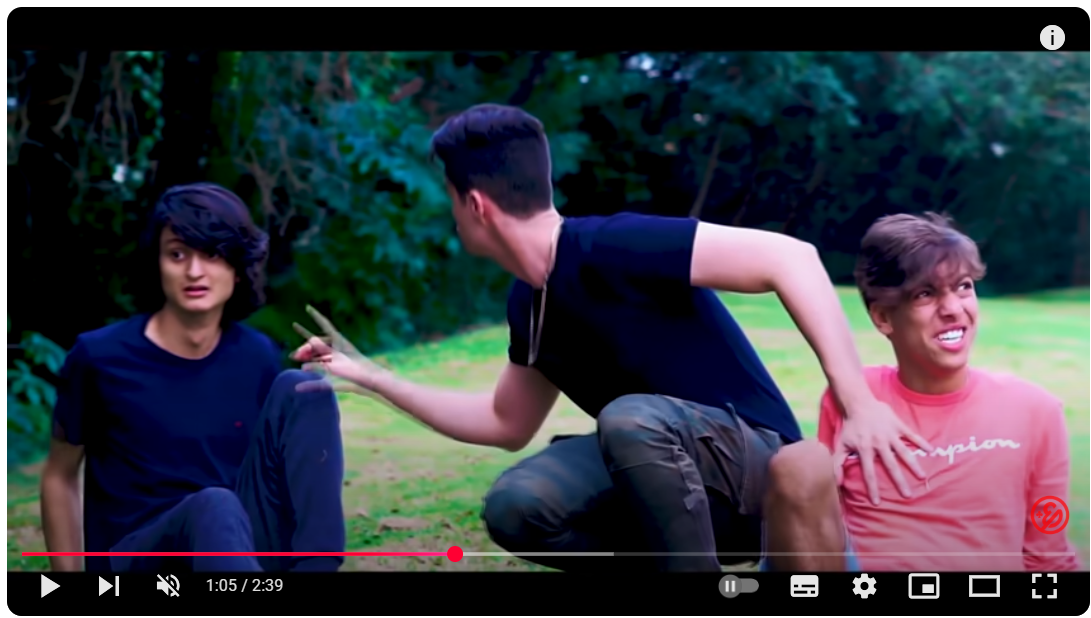
\includegraphics[width=\textwidth]{fig+005.png}
 \caption{Print do vídeo “Não fale o nome do Monstro”.Fonte: canal Enaldinho.}
 \label{fig5}
 \source{\textcite{enaldinho2025naofale}.}
\end{minipage}
\end{figure}

Na letra da canção, temos o seguinte:

\begin{quote}
    Não fale o nome do monstro/ Vai que ele aparece
    
Não fale o nome do monstro/ Uns dizem que ele chama Zap

Cuidado com o monstro / Não chame seu nome

Ele é feio / Mais feio que a fome
\\
\\
Cheio de armadilhas / ele não é bobo

O monstro te pega / E te propõe um jogo

Será que é vampiro? / Tem medo de alho?

Será a carta / Mais forte do baralho?
\\
\\
O bicho é traíra / Cheio de ciladas

Ele já sequestrou /Minha namorada […]
\\
\\
Foi a gota d’água / Tô cheio de pistas

Cuidado que o monstro / Se multiplica

Ele aparece / Se o seu nome chama

Será que ele vive / debaixo da cama?

Transcrição da letra da canção “Não fale o nome do monstro”.
\cite{enaldinho2025naofale}.
\end{quote}

Na letra da canção, o monstro Zap guarda similaridade com a mitologia popular do “bicho papão”. A imagem do tal monstro é uma cópia do Huggy Wuggy, mencionado anteriormente, monstro de outro canal infantil no Youtube, estadunidense e que viralizou também no Brasil. Através dele, Enaldinho consegue criar uma filiação estética com o canal em questão, este também popular entre o público infantil. O vídeo está povoado por referências a outros conteúdos infantis, configurando processos de \textit{intertextualidade} e \textit{autorreferenciação}, o que permite criar relações entre a identidade de Enaldinho e a de outros canais infantis, dissimulando proximidade e identificação com o público infantil (\Cref{fig6}).

\begin{figure}[htbp]
\centering
\begin{minipage}{.8\textwidth}
 
\includegraphics[width=\textwidth]{fig-006.png}
 \caption{O monstro Zap no videoclipe “Não fale o nome do Monstro”.}
 \label{fig6}
 \source{\textcite{enaldinho2025naofale}.}
\end{minipage}
\end{figure}

Ainda na letra, no trecho “O bicho é traíra / Cheio de ciladas / Ele já sequestrou /Minha namorada”, Enaldinho refere-se a outro vídeo da websérie em que o monstro Zap sequestra Aninha, a namorada de Enaldinho, que participa frequentemente de vídeos no canal e cuja imagem corporal figura nos termos em que o entretenimento para adultos tende a objetificar mulheres (\Cref{fig7}).

\begin{figure}[h!]
\centering
\begin{minipage}{.8\textwidth}
 
\includegraphics[width=\textwidth]{fig-007.png}
 \caption{Print da capa de “O Zap Sequestrou Minha Namorada!”.}
 \label{fig7}
 \source{\textcite{enaldinho2025zap_sequestrou}.}
\end{minipage}
\end{figure}

Enquanto podemos atribuir, se inflamados pela perspectiva crítica, uma certa perversidade no ato de expor crianças ao velho discurso da objetificação feminina, ao mesmo tempo temos um \textit{influencer} inserido no modelo de negócio dos influenciadores e da cultura de \textit{influencer}, que consiste nisso mesmo: o autorreferenciamento narcísico que, por sua ubiquidade nas redes sociais, é naturalizado ao ponto de se tornar invisível à primeira vista. Não é novidade que a ostentação passe por exibir corpos femininos no padrão de beleza como se exibe um carro, por exemplo. Na figura da namorada como parte do conteúdo, Enaldinho nos mostra que essa canção infantil é, também, um esforço retórico de autopromoção.

Na narrativa de herói encenada no vídeo, o monstro Zap ainda rouba o Porsche de Enaldinho. Apesar de não estar contido no videoclipe, Enaldinho tem numerosos vídeos sobre seu carro, que atua com o peso de um personagem em suas narrativas infantis. Não se trata, evidentemente, de uma mera subtração material, mas da desapropriação simbólica de um dos elementos mais distintivos do \textit{youtuber} e um totem narrativo dentro do universo que constrói para seu público infantil (\Cref{fig8}).

\begin{figure}[htbp]
\centering
\begin{minipage}{.8\textwidth}
 
\includegraphics[width=\textwidth]{fig-008.png}
 \caption{Print da capa do vídeo “O Zap Roubou Minha Porsche!”. Fonte: canal Enaldinho.}
 \label{fig8}
 \source{\textcite{enaldinho2025zap}.}
\end{minipage}
\end{figure}

O Porsche não é um apenas meio de transporte, mas um dispositivo narrativo \cite[p. 19]{Gulino2004Screenwriting}: representa um símbolo de \textit{status} que é ao mesmo tempo acessível e inalcançável para o público infantil, inserindo o desejo de consumo dentro do universo ficcional do canal. Sua presença em múltiplos vídeos não apenas reforça a identidade de Enaldinho como um indivíduo bem-sucedido (este performado para uma audiência que sequer atingiu a idade mínima para conduzir veículos), mas também insere um símbolo de status adulto em um espaço lúdico, revestindo-o com um verniz de encantamento. Trata-se, em última instância, da domesticação do fetiche da mercadoria para o universo infantil: se a literatura fantástica desde sempre faz crianças sonharem com objetos mágicos e talismãs encantados, no YouTube esse imaginário é reformulado sob o molde da cultura de \textit{influencer}, oferecendo como horizonte de desejo não mais a transcendência de um mundo ordinário pela via do maravilhoso, mas a sedução pelo consumo, estabelecendo dentro do brincar infantil a mesma premissa ideológica-hegemônica das fantasias de consumo dos adultos. Em Enaldinho, o limite entre o fascínio fantástico e a assimilação da ideologia se traduzem, tanto para adultos quanto para crianças, no brilho quase mítico de um carro esportivo.

Temos, ainda, o fenômeno discursivo do \textit{ethos} adulto manifesto na narrativa: a transmutação de um objeto de consumo em um artefato dotado da mesma aura de excepcionalidade que uma varinha mágica ou uma lâmpada encantada, cuja posse ou privação estabelece os contornos da trama construída na \textit{websérie} sobre o monstro Zap.

Ao longo desta análise, a construção do \textit{ethos discursivo} de Enaldinho dialoga com os demais processos e recursos semiótico-discursivos, mostrando um esforço meticuloso na construção e negociação da identidade do \textit{youtuber} nos múltiplos significantes modais e na articulação entre eles. A \textit{identidade de estilo} do videoclipe analisado, bem como a do \textit{youtuber} como figura pública, está em um híbrido entre o infantil e o adulto, e gera um campo entre a infância encenada e a posição de influenciador bem-sucedido em que, ao invés de contraditórias, funcionam juntas, validando-se mutuamente.

Nessa análise do vídeo, identificamos modos semióticos que se abrigam dentro do modo kineicônico, cada qual realizando uma operação discursiva, com sua respectiva finalidade interacional (\Cref{tab3}).

\begin{table}[htbp]
\centering
\begin{threeparttable}
\caption{Descritivo de recursos discursivos operados no vídeo}
\label{tab3}

\begin{tabularx}{\textwidth}{
>{\raggedright\arraybackslash}p{3.5cm}
>{\raggedright\arraybackslash}p{2.5cm}
>{\raggedright\arraybackslash}p{3.2cm}
X}
\toprule
Descrição &
Modos &
Finalidade interacional &
Recurso \\
\midrule

Música: letra da canção &
Verbal oral &
Narrar história &
Autorreferenciação; intertextualidade; construção de \textit{ethos} adulto; construção de \textit{ethos} infantil \\

Música: instrumental &
Sonoridade &
Musicalizar narrativa &
Construção de \textit{ethos} adulto \\

Vídeo &
Imagem em movimento &
Visualização da narrativa &
Autorreferenciação; intertextualidade; construção de \textit{ethos} adulto; construção de \textit{ethos} infantil \\

Expressões faciais &
Gestual &
Expressão &
Construção de \textit{ethos} infantil \\

Figurino &
Imagético &
Caracterização &
Construção de \textit{ethos} adulto \\

Penteado &
Imagético &
Caracterização &
Construção de \textit{ethos} infantil \\

Personagens coadjuvantes &
Imagético &
Suporte à narrativa &
Construção de \textit{ethos} infantil \\

Capa final do vídeo &
Imagético &
Direcionar a outros vídeos &
Hiperlinkagem; intertextualidade \\

\bottomrule
\end{tabularx}

\source{Own elaboration.}

\end{threeparttable}
\end{table}
Em síntese, o sucesso discursivo de Enaldinho parece residir na sua capacidade de navegar entre diferentes polos identitários, equilibrando infantilização, aspiração ao consumo e uma comunicação intertextual potencialmente eficaz. O resultado é um ethos híbrido, fruto de um processo de constante negociação e dosagem, e distribuído estrategicamente entre os modos semióticos constituintes da \textit{affordance} do Youtube.

\section{Considerações finais}\label{sec-organizacao}
Neste artigo, apresentamos os resultados preliminares da pesquisa \textit{A brincadeira do invisível: recursos discursivos multimodais no entretenimento infantil mediado pelo Youtube}, cujo objetivo é analisar processos, significados e modos de ação, interação e relação social e discursiva em vídeos de entretenimento infantil no YouTube brasileiro. Estudamos o impacto potencial do algoritmo do YouTube sobre o conteúdo infantil produzido e veiculado pela plataforma digital, partindo da Análise de Discurso Crítica \cite{Fairclough2003AnalysingDiscourse,VieiraResende2016AnaliseDiscursoCritica,Vieira2024Decolonial} e apresentando a análise discursivo-semiótica da página do vídeo “Não fale o nome do monstro”, do Canal YouTube Enaldinho, com foco em processos multissemiótico-discursivos principais como: affordance, indexação, metaconteúdo, estruturas visuais e esquema modular, ethos discursivo, intertextualidade \cite{Benson2016DiscourseYouTube,ColetivaCiborga2022EtnografiaDigital,Fairclough2003AnalysingDiscourse,KressVanLeeuwen2020ReadingImages,Maingueneau2020GenerosWeb}.

O exemplar de vídeo analisado ilustra o que é recorrente no \textit{corpus} de dados completo: o \textit{ethos} é construído de forma a promover um processo de adultização do conteúdo infantil, incorporando características discursivas e performativas típicas da cultura \textit{influencer}. Essa dinâmica inter-acional e relacional discursiva aproxima o universo infantil de estilos comunicacionais e aspiracionais próprios do público adulto, tensionando os limites entre infância e experiência digital contemporânea, a serviço da adultificação do conteúdo infantil conforme as demandas e especificidades do meio digital.

De forma reiterada, as ações, interações e relações interpessoais possibilitadas pela plataforma a apontam como agente estruturante e, assim, coautora dos discursos que veicula. Por isso, debatemos como a \textit{affordance} atua como vetor fundamental na produção, composição, circulação e leitura de um gênero discursivo situado característico do YouTube, de natureza multimodal, responsiva e performativa.

Ademais, os já conhecidos movimentos retóricos da mídia como entidade reguladora do simbólico (adultificação, autopromoção) encontram no ambiente digital um terreno fértil, mais responsivo, mais imersivo, mais personalizado. Podemos falar, sim, de uma aceleração dos processos mediáticos extravirtuais quando no mundo \textit{online}, tanto no paradigma de interação entre atores sociais quanto das demandas mercadológicas do entretenimento.

Esperamos contribuir para o avanço teórico-metodológico dos estudos discursivos críticos sobre infância e plataformas digitais; para investigações sobre infância, multimodalidade e a regulação do simbólico nas plataformas digitais e, ainda, análises multimodais desse tipo de material digital em práticas de ensino-aprendizagem.


\printbibliography\label{sec-bib}
% if the text is not in Portuguese, it might be necessary to use the code below instead to print the correct ABNT abbreviations [s.n.], [s.l.]
%\begin{portuguese}
%\printbibliography[title={Bibliography}]
%\end{portuguese}


%full list: conceptualization,datacuration,formalanalysis,funding,investigation,methodology,projadm,resources,software,supervision,validation,visualization,writing,review
\begin{contributors}[sec-contributors]
\authorcontribution{Helena Sarmento Barros}[conceptualization,formalanalysis,investigation,methodology,writing]
\authorcontribution{Viviane Cristina Vieira}[conceptualization,methodology,resources,supervision,writing,review]
\end{contributors}

\begin{dataavailability}
\txtdataavailability{databody} % options: dataavailable, dataonly, databody, datanotav, nodata
\end{dataavailability}

\begin{funding}
Esta publicação foi realizada com o apoio da Fundação de Apoio à Pesquisa do Distrito Federal (FAP-DF).
\end{funding}




\end{document}

